\documentclass{article}

     \usepackage[nonatbib]{neurips_2020}

\usepackage[utf8]{inputenc} % allow utf-8 input
\usepackage{subfigure}
\usepackage[T1]{fontenc}    % use 8-bit T1 fonts
\usepackage{hyperref}       % hyperlinks
\usepackage{url}            % simple URL typesetting
\usepackage{booktabs}       % professional-quality tables
\usepackage{amsfonts}       % blackboard math symbols
\usepackage{nicefrac}       % compact symbols for 1/2, etc.
\usepackage{microtype}      % microtypography
\usepackage{graphicx,booktabs,multirow}

\title{Admission Data Prediction Using Machine Learning Methods}


\author{
  Zhaozheng Shen\\ 
Shanghaitech \\
\texttt{shenzhzh} \\
  % Address \\
  % \texttt{email} \\
\AND
Wenke Jing \\
Shanghaitech \\
11120602\\
\texttt{jingwk} \\
}

\begin{document}

\maketitle

\begin{abstract}
Nowadays, graduate admission becomes the most popular problem for graduates. In this project, we use a variety of machine learning algorithms to solve this problem. After analysis the running time and accuracy, we achieved the accuracy to $78.377\%$.
\end{abstract}

\section{Introduction}
As students, we care a lot about the graduate admissions problem and there isn't any work done in the past. We choose a dataset created for prediction of Graduate Admissions from an Indian perspective, which predicting admission from $7$ important parameters with $500$ students. [1] The output of our problem is a number from $0$ to $1$, which represents the probably a student being admitted. After preprocessing the data, we use $11$ machine learning methods to deal with this problem and analyze the performance including RSS error, accuracy and running time of these methods.

\section{Methodology}

\subsection{Preprocessing}
Firstly, we do the data splitting process, we randomly divide 500 input data into three parts: 320 train data, 80 validation data, and 100 testing data.
Secondly, we do subset selection to find the best subset of 7 feature parameters. Then, we normalize the input data before loading them into algorithm models.
Additionally, some algorithm may not support regression task, such as logistic regression, LDA, and Naive Bayes, so for these algorithm, we change the regression task into classification task by approximating the output number into 10 neighbor classes.

\subsection{Algorithm}

\textbf{Least square} Fit a linear model with coefficients $w = (w_1, ..., w_p)$ to minimize the sum of squared residuals between the actual observed data and the predicted data (estimated values) of the data set: $min_w ||Xw-y||_2^2$.\\
\textbf{Ridge regression} Ridge regression solves some problems of ordinary least squares by penalizing the size of the coefficients. What minimizes the ridge coefficiet is the sum of squared residuals with penalties: $min_w ||Xw-y||_2^2+\alpha ||w||_2^2$.\\
\textbf{Lasso regression} Lasso regression consists of a linear model with regular terms of $l_1$-norm. Its minimized objective function is: $min_w \frac{1}{2n_{samples}} ||Xw-y||_2^2+\alpha ||w||_1$. [2]\\
\textbf{Knn} Knn is also a regression method, it is used when the data labels are continuous variables rather than discrete variables. The label assigned to the query point is calculated from the average of its nearest neighbor labels. [3]\\
\textbf{Decision tree} The nearest neighbor regression is used when the data labels are continuous variables rather than discrete variables. The label assigned to the query point is calculated from the average of its nearest neighbor labels.\\
\textbf{SVM} It is very efficient in high-dimensional space, and different kernel functions have a one-to-one correspondence with specific decision functions. Common kernels are already provided, and custom kernels can also be specified. [4]\\
\textbf{Boosting} The goal of the boosting method is to combine the prediction results of multiple base estimators constructed using a given learning algorithm to obtain better generalization ability/robustness than a single estimator. We mainly focus on Random Forest and AdaBoost. [5]\\
\textbf{LDA} This is a classification method. It is derived from simple probability models, and these models can be obtained by Bayes' theorem for the relevant distribution $P(X|y=k)$ of each category k.
\textbf{Naïve Bayes} This is a classification method. Naive Bayes methods are a set of supervised learning algorithms based on applying Bayes’ theorem with the “naive” assumption of conditional independence between every pair of features given the value of the class variable. [6]\\
\textbf{Logistic} This is a classification method. Logistic regression is a generalized linear model, so it has many similarities with multiple linear regression analysis. Their model form is basically the same. It gets dependent variable value by logistic function.

\section{Experiment}
\label{headings}

\subsection{Preprocessing}

In the preprocessing process, after splitting data into training, validation and testing data, and before normalization, we do subset selection to find the best subset of 7 feature parameters. During subset selection, For each $s \in 0, 1, ... , p$, find the subset in size of $s$ that gives lowest RSS, and use cross-validation to esitimate prediction error and select $s$. Then, we can select the optimal variables. The result is showed below. We can learn from the result that the best subset is the total set, we do not need to filter any feature parameter. In addition, it is quite friedly for us to use the moethod to selection the best subset, since it need a lot of computation and a lot of time when $p$ is too large, but our $p$ is $7$, and the dataset is small, so the running time is not too long.
\begin{figure}[htbp]
\centering
\subfigure[subset selection]{
\begin{minipage}[t]{0.3\linewidth}
\centering
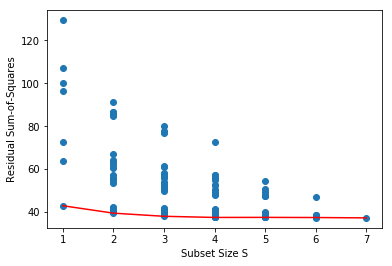
\includegraphics[width=1.5in]{preprocessing2.jpg}
%\caption{fig1}
\end{minipage}%
}%
\subfigure[subset selection]{
\begin{minipage}[t]{0.3\linewidth}
\centering
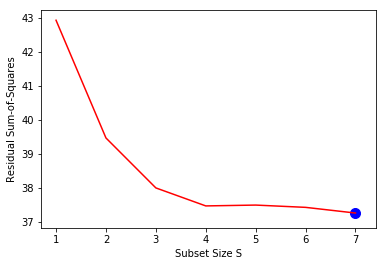
\includegraphics[width=1.5in]{preprocessing.jpg}
%\caption{fig2}
\end{minipage}%
}%
\subfigure[linear regression]{
\begin{minipage}[t]{0.3\linewidth}
\centering
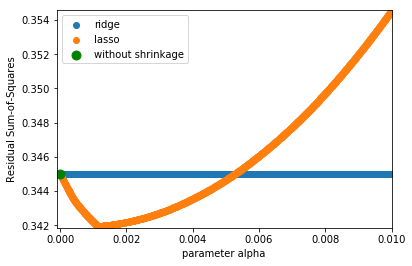
\includegraphics[width=1.5in]{linear_regression.jpg}
%\caption{fig2}
\end{minipage}
}%
\centering
\end{figure}
\subsection{Algorithm Result}
\paragraph{Regression}
First, we use regression algorithm to fit the admission rate. We use without shrinkage, lasso and ridge models to find the best model, by optimizing the parameter alpha through the analysis of RSS error. Alpha indicates the degree of shrinkage. When alpha approaches 1, it indicates that the degree of shrinkage reaches its maximum; when alpha approaches 0, it indicates that there is no shrinkage.
The RSS of the three methods varies with alpha are shown in figure (c). It can be seen that the smallest RSS is at lasso regression, and alpha at this time is 0.3419, test accuracy is $78.377\%$.


\paragraph{Decision Tree}
In decision tree algorithm, we find the optimal model by finding at which depth we will get the lowest RSS in validation set.
From Figure (d) we can know that we can get the lowest RSS at $depth = 4$, and the RSS value is $0.4518$. The test accuracy of this method is $74.015\%$.


\paragraph{KNN}
Using KNN regression, we need to find the optimal $k$ value. We want to find at which $k$ value we will get the lowest RSS in validation set. From Figure (e) we can know that we can get the lowest RSS at $k=31$, and the RSS value is $0.3546$. The test accuracy of this method is $66.657\%$.



\paragraph{SVM}
In SVM regression method, we can apply different kernel on it. The min error without any kernel is $0.5596$. As shown in figure (f), best rbf kernel the lowest RSS in validation set at $gamma =5.0351e-05$, and the RSS value is $0.4495$, the validation accuracy of this method is $61.790\%$. As shown in figure (g), best linear kernel with the lowest RSS in validation set at $C=0.0918$, and the RSS value is $0.4476$, the validation accuracy of this method is $62.210\%$. Best poly kernel with the lowest RSS in validation set at $degree=1$, and the RSS value is $0.4532$, the validation accuracy of this method is $62.110\%$.


\paragraph{AdaBoost}
When we using AdaBoost method, we are using a lot of weak estimators to regress this problem. So we want to find the optimal number of the weak estimators. As shown in figure (h), the lowest RSS in validation set at the $n\_estimators =10$, and the RSS value is $0.3982$, the test accuracy of this method is $65.844\%$. At the same time, we realized that the running time may have some relation with the number of the weak estimators, and then we record the running time of this method with different number of the weak estimators. As shown in figure (i), the running time increases as the number of the weak estimators increases. We can get the conclusion that the optimal RSS may not correspond with the shortest running time. And we want to choose a n\_estimaters parameter, we cannot choose a really large number which may make the running time really large.

\paragraph{Random Forest}
We need to find the optimal model by finding the optimal n\_estimators and optimal depth, by get the lowest RSS in validation set. Firstly, figure (j), we choose best n\_estimators by running model with different n\_estimators and choose the best. But during this process, we find out as n\_estimators increase, the time that cost to run the algorithm increase linearly (figure (k)), so its not elegant to choose large n\_estimators. After finding the optimal n\_estimators, we start finding the optimal depth with optimal n\_estimators. Also, the model start overfitting at $depth = 3$. From Figure (l) we know that we can get the lowest RSS in the validation set at $depth = 4$, $n\_estimators = 13$, and the RSS value is $0.3797$. Test accuracy of this method is $74.522\%$.
\begin{figure}[htbp]
\centering
\subfigure[decision tree]{
\begin{minipage}[t]{0.3\linewidth}
\centering
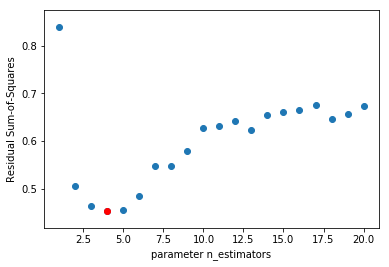
\includegraphics[width=1.5in]{decision_tree.jpg}
%\caption{fig1}
\end{minipage}%
}%
\subfigure[KNN]{
\begin{minipage}[t]{0.3\linewidth}
\centering
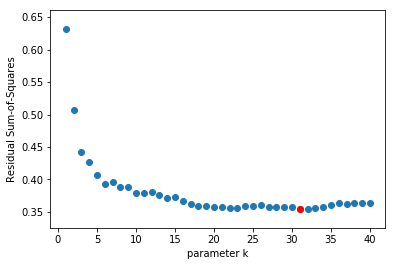
\includegraphics[width=1.5in]{knn.jpg}
%\caption{fig2}
\end{minipage}%
}%
\subfigure[svm]{
\begin{minipage}[t]{0.3\linewidth}
\centering
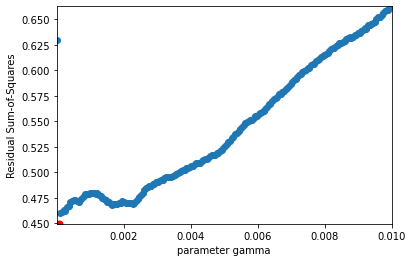
\includegraphics[width=1.5in]{svm1.jpg}
%\caption{fig2}
\end{minipage}
}%
\centering
\end{figure}
\begin{figure}[htbp]
\centering
\subfigure[svm]{
\begin{minipage}[t]{0.3\linewidth}
\centering
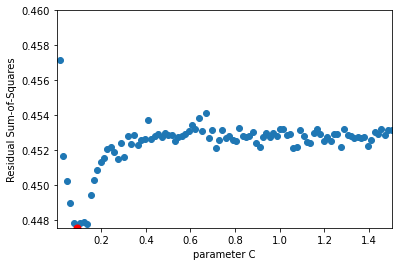
\includegraphics[width=1.5in]{svm2.jpg}
%\caption{fig1}
\end{minipage}%
}%
\subfigure[AdaBoost]{
\begin{minipage}[t]{0.3\linewidth}
\centering
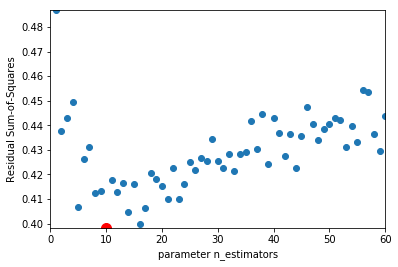
\includegraphics[width=1.5in]{adaboost1.jpg}
%\caption{fig2}
\end{minipage}%
}%
\subfigure[AdaBoost]{
\begin{minipage}[t]{0.3\linewidth}
\centering
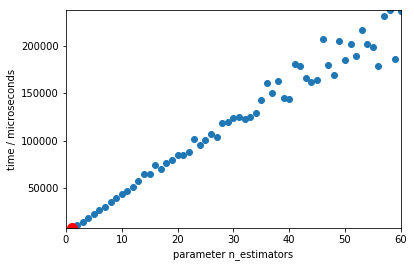
\includegraphics[width=1.5in]{adaboost2.jpg}
%\caption{fig2}
\end{minipage}
}%
\centering
\end{figure}

\begin{figure}[htbp]
\centering
\subfigure[random forest]{
\begin{minipage}[t]{0.3\linewidth}
\centering
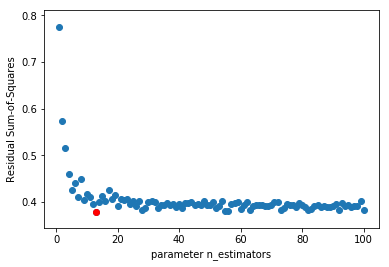
\includegraphics[width=1.5in]{random_forest1.jpg}
%\caption{fig1}
\end{minipage}%
}%
\subfigure[random forest]{
\begin{minipage}[t]{0.3\linewidth}
\centering
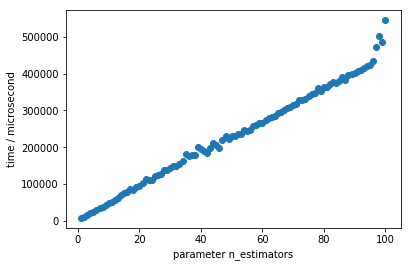
\includegraphics[width=1.5in]{random_forest2.jpg}
%\caption{fig2}
\end{minipage}%
}%
\subfigure[random forest]{
\begin{minipage}[t]{0.3\linewidth}
\centering
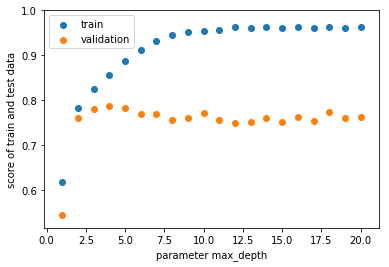
\includegraphics[width=1.5in]{random_forest3.jpg}
%\caption{fig2}
\end{minipage}
}%
\centering
\end{figure}


\paragraph{Classification Methods}
Besides the regression method above, we also use some classification methods to solve this problem.\\
\textbf{Logistic} When we try different penalty function, we find that $l_1$ function is a little bit better than $l_2$. The lowest RSS in validation set is $0.7880$, and the test accuracy is $52.500\%$.\\
\textbf{Naïve Bayes} Comparing Gaussian NB and Bernoulli NB, we find that Gaussian NB has better effect. The lowest RSS in validation set is $0.7$, and the test accuracy is $58.750\%$.\\
\textbf{LDA} The LDA method with default solver $svd$ can reach the test accuracy $51.250\%$, and the lowest RSS in validation set is $0.5440$.



\subsection{Analyze and Compare different methods}
\begin{table}
	\caption{Performances}
	\label{sample-table}
	\centering
	\begin{tabular}{ccccccccc}
		\toprule
		Algorithm     & RSS error     & Val Accuracy  & Test Accuracy & Time(Microsecond)\\
		\midrule
		Regression(Lasso) & \textbf{0.3419}  & \textbf{88.956\%} & \textbf{78.377\%} & \textbf{1293}    \\
		KNN     & \textbf{0.3546} & 77.199\%   & 66.657\% & 3089  \\
		Decision Tree     & 0.4518       & 81.410\%  & \textbf{74.015\%} & \textbf{867}\\
		SVM(Linear)     & 0.4476      & 76.862\% & 54.370\% & 3122\\
		AdaBoost     & 0.3982       & \textbf{81.611\%} & 65.844\% & 9639\\
		Random Forest    & \textbf{0.3797}       & \textbf{84.684\%} & \textbf{74.522\%} & \textbf{11593} \\
		LDA   & 0.5440       & 66.667\% & 51.250\% & 1400\\
		Naive Bayes(Gaussian)    & 0.7000       & 64.286\% & 58.750\% & 1599 \\
		Logistic(L1-penalty)    & 0.7880       & 58.333\%  &52.500\% & 4017\\
		\bottomrule
	\end{tabular}
\end{table}
\textbf{Test Accuracy}
The regression (Lasso) performance very well in the test data, it can reach $78.377\%$ accuracy which is the highest in all methods above. It fits for data with linear relationship well which is similar to our dataset. Because of its simple implementation and simple calculation, the running time is short, and this is also a good performance.
\\Random forest and Decision tree also has a high accuracy in test data, this kind of method is easy to understand and able to deal with unrelated features and make feasible and good results for large data sources in a relatively short time. But it may have some overfitting problems.\\
\textbf{Overfitting}
We can find some obvious overfitting problems in SVM and AdaBoost, there is a big difference between their val accuracy and test accuracy. The overfitting in SVM may due to the required interval too large, that is, when the parameter of C in the soft-space support vector machine is too large, it means that the interval is more important and the data is completely separated. When C tends to infinity, it is equivalent to a hard-interval SVM. In general, AdaBoost shouldn't have overfitting problem because of the weak estimators are simple, however, we indeed has this problem in our experience which we think the weak estimators are not simple enough may cause this consequence.\\
\textbf{Running time}
As for time, we notice that decision tree is very fast, and the two boosting algorithms(AdaBoost and Random Forest) are quite slow. The efficiency of the decision tree is high, it only needs to be constructed once and used repeatedly, and the maximum calculation times of each prediction does not exceed the depth of the decision tree. However, in boosting algorithms, different classification algorithms can be used as weak classifiers, which make good use of weak classifiers for cascading, but the training is time-consuming.



\section{Conclusion}
In this project, we focus on the problem that predicting the probability a student being admitted. We used eleve machine learning algorithms to solve this problem, and analyze the performance including RSS error, accuracy and running time. From our results, we find that regression with lasso and decision tree are good methods since they can guarantee speed while maintaining good performance. In addition, although the accuracy of random forest is good, it takes a long time. If we want to continue working on this project, we will focus on trying different loss functions, and enlarge dataset to overcome the overfitting problem.\\
Contribution: Znaozheng Shen contributes Decision Tree, Random Forest, Naïve Bayes; Wenke Jing contributes AdaBoost, Logistic, LDA. And the others together.
\section*{References}


\small
[1] Mohan S Acharya, Asfia Armaan, Aneeta S Antony : A Comparison of Regression Models for Prediction of Graduate Admissions, IEEE International Conference on Computational Intelligence in Data Science 2019

[2] “Regularization Path For Generalized linear Models by Coordinate Descent”, Friedman, Hastie \& Tibshirani, J Stat Softw, 2010

[3]  “Multidimensional binary search trees used for associative searching”, Bentley, J.L., Communications of the ACM (1975)

[4] Fan, Rong-En, et al., “LIBLINEAR: A library for large linear classification.”, Journal of machine learning research 9.Aug (2008): 1871-1874.

[5] [FS1995] Y. Freund, and R. Schapire, “A Decision-Theoretic Generalization of On-Line Learning and an Application to Boosting”, 1997.

[6] H. Zhang (2004). The optimality of Naive Bayes. Proc. FLAIRS.
\end{document}
